\chapter{Planejamento do projeto}

Nesta seção será abordado um cronograma que a equipe se baseou para a realização das atividades até a data de entrega deste documento. Nesse cronograma estão destacadas as datas de entrega das atividades e os responsáveis por cada uma delas, isso torna mais fácil o contato com a pessoa que realizou a atividade caso a mesma precise de alguns ajustes.

\section{Cronograma}

	O cronograma a seguir mostra quais as atividades foram executadas pela equipe, além de quais recursos humanos e de tempo foram alocados para execução dos mesmos. Foi utilizado o Gantter que é uma ferramenta para gestão de projetos open-source.

	\begin{figure}[!htpb]
	\centering
	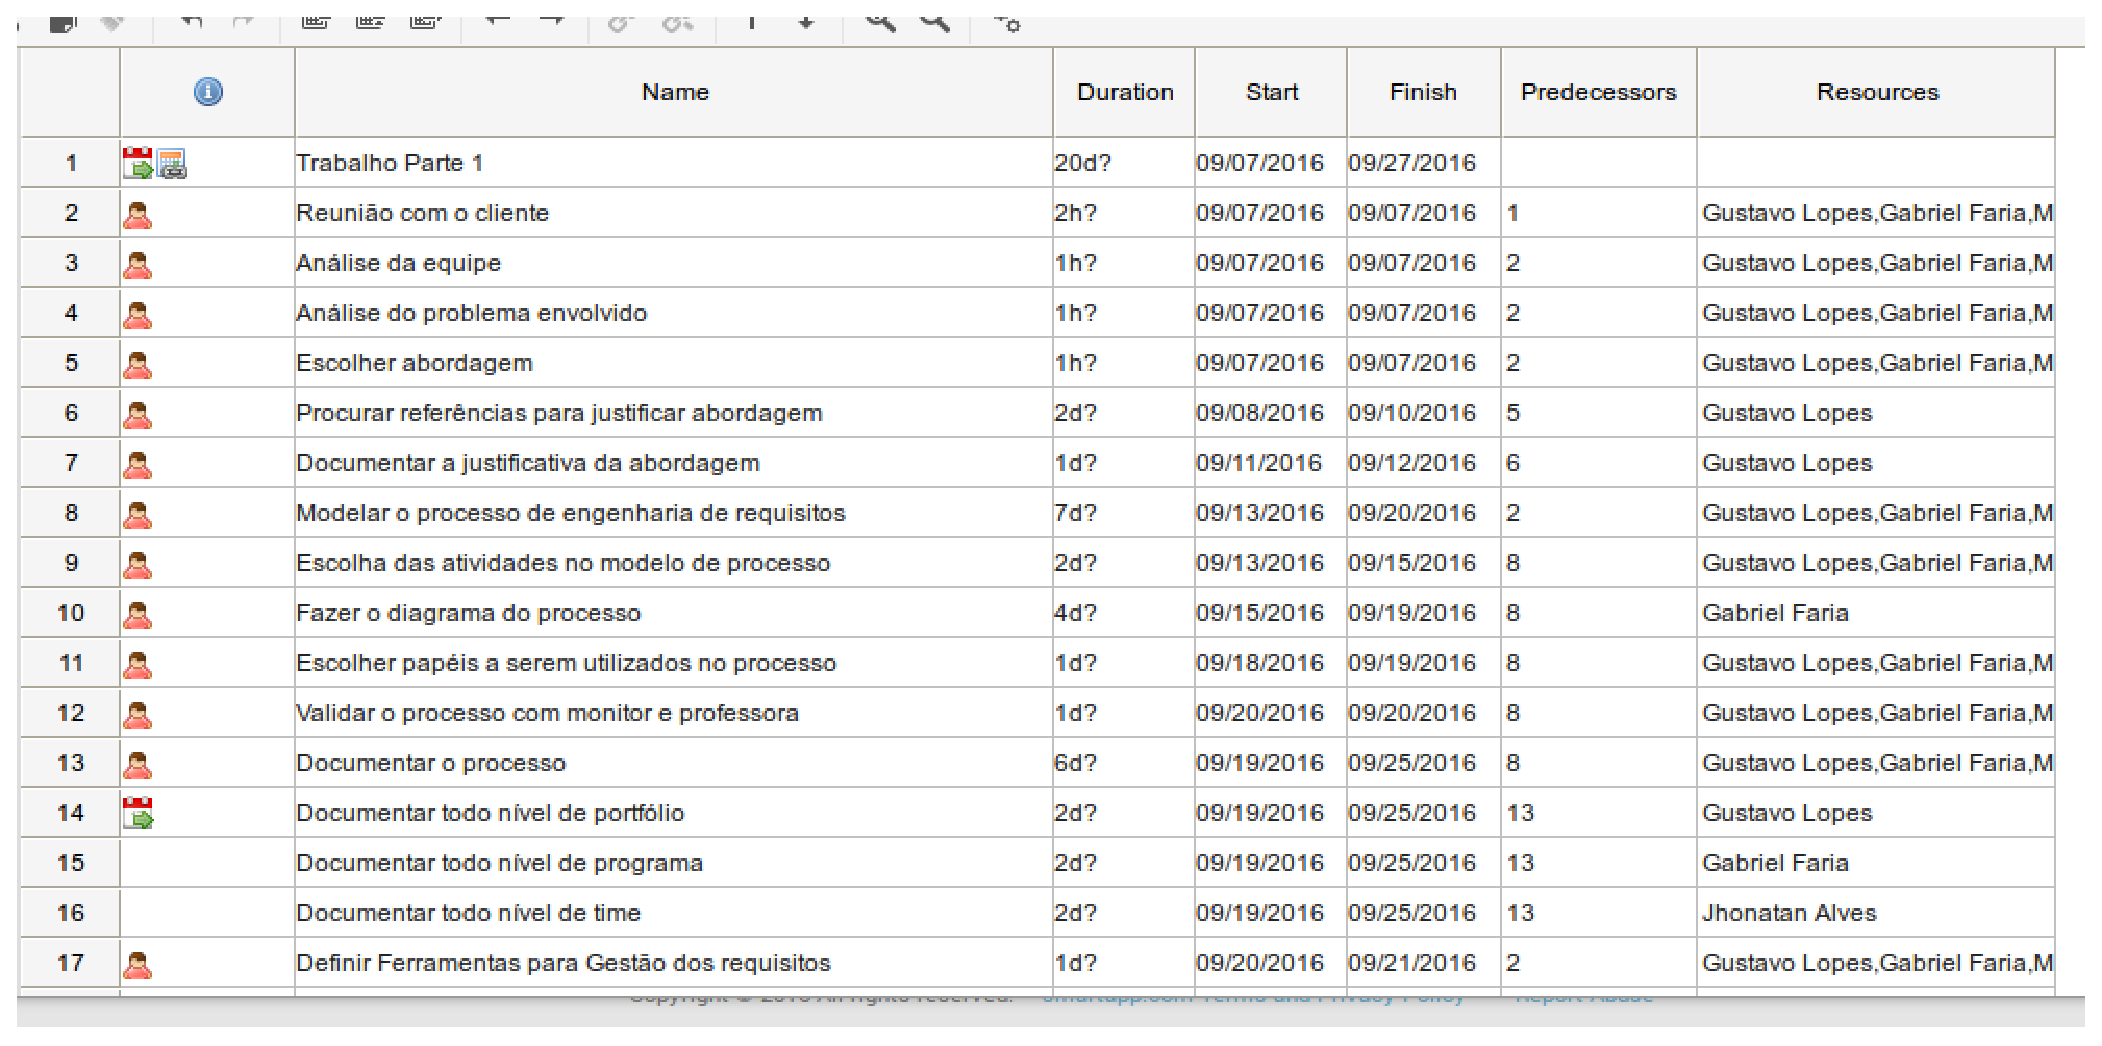
\includegraphics[scale=0.4]{figuras/cronograma/parte1}
	\caption{Exibição do cronograma e suas atividades e durações}
	\end{figure}

	\begin{figure}[!htpb]
	\centering
	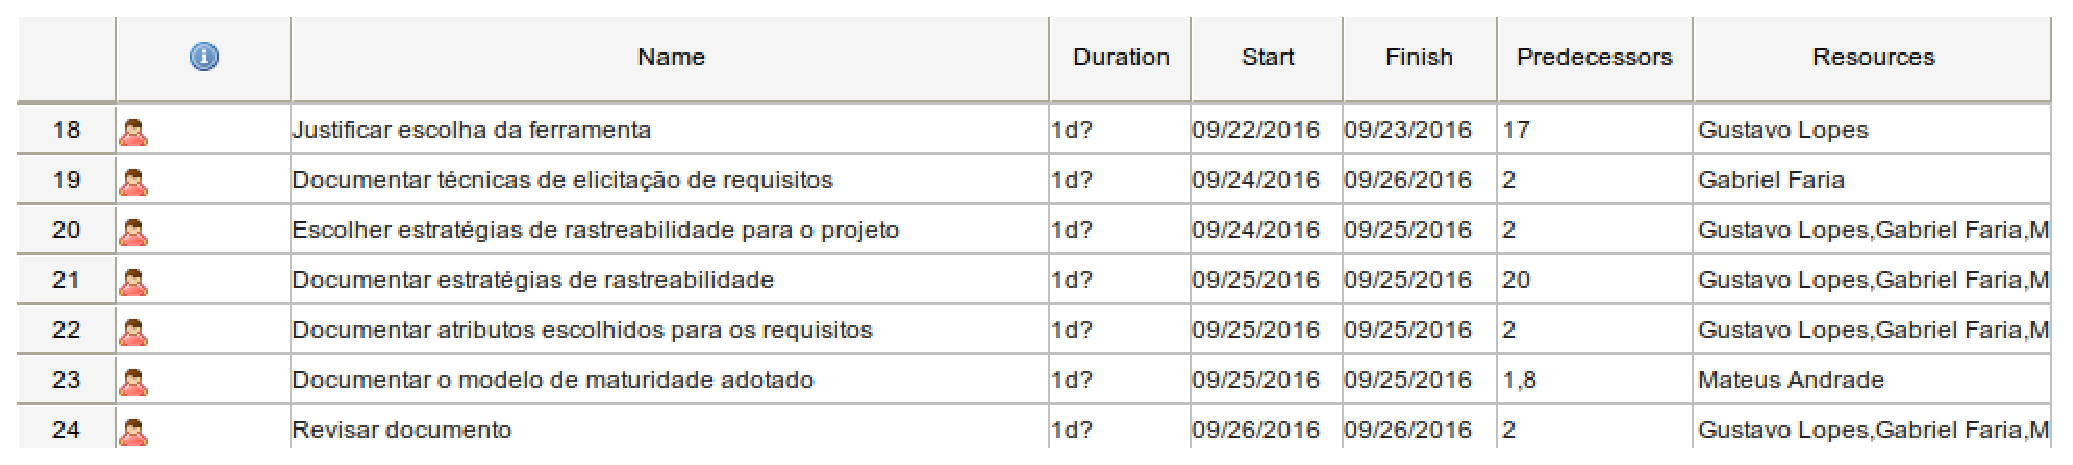
\includegraphics[scale=0.4]{figuras/cronograma/parte2}
	\caption{Parte 2 do cronograma}
	\end{figure}

\section{Fases}
	O ciclo de vida do projeto foi dividido em três fases, a fase de iniciação, a de planejamento e a de execução.

\subsection{Fase de iniciação}
Essa fase consiste nas atividades iniciais do desenvolvimento do projeto. Foi realizada a primeira reunião com o cliente que influenciou na escolha da metodologia a ser utilizada.
\begin{itemize}
\item Data de início: 7 de Setembro
\item Data de término: 11 de Setembro
\item Status: Concluída
\end{itemize}

\subsection{Fase de Planejamento}
Essa fase consiste nas propostas feitas pela primeira parte do projeto, baseando-se no framework SAFe para modelar o processo que envolve uma maneira de trabalhar com a metodologia ágil. As atividades desenvolvidas nessa fase serão essenciais para a fase de execução, já que o processo modelado será executado nesse próximo momento.
\begin{itemize}
\item Data de início: 12/09/2016
\item Data de término: 27/09/2016
\item Status: Concluída
\end{itemize}

\subsection{Fase de Execução}
Nesta fase, se dará a execução do processo modelado para resolução do problema apresentado pelo cliente Padaria da Vila, através de um software para controle de estoque e desperdício, o mesmo será construído utilizando do modelo adotado e uso das ferramentas para gestão e rastreabilidade dos requisitos.
\begin{itemize}
\item Data de início: 28/09/2016
\item Data de término: 30/11/2016
\item Status: Não iniciada
\end{itemize}